\documentclass[conference]{IEEEtran}
\usepackage{graphicx}
\graphicspath{ {images/} }
\DeclareRobustCommand*{\IEEEauthorrefmark}[1]{%
	\raisebox{0pt}[0pt][0pt]{\textsuperscript{\footnotesize #1}}%
}

\begin{document}

\title{ARchitect: AR Based Construction Simulator}

\author{\IEEEauthorblockN{
		\IEEEauthorrefmark{1}L. Sai Kiran Reddy,
		\IEEEauthorrefmark{2}Vijay Krishna Vallabhaneni, 
		\IEEEauthorrefmark{3}M. Kesava Krishna Reddy,
		\IEEEauthorrefmark{4}L. Satish Kumar and
		\IEEEauthorrefmark{5}Elakya R	
}
	\IEEEauthorblockA{\IEEEauthorrefmark{1234}UG Scholars
		\IEEEauthorrefmark{5}Assistant Professor (Guide)
	}
	
		
	\IEEEauthorblockA{Department of Computer Science and Engineering\\
	SRMIST, Ramapuram, Chennai, India}
	\IEEEauthorblockA{Email: \IEEEauthorrefmark{1}saikiranreddy1001@gmail.com,
\IEEEauthorrefmark{2}krsnvijay@gmail.com,
\IEEEauthorrefmark{3}m.k.k.r.332@gmail.com,\\
\IEEEauthorrefmark{4}satishaaa111@gmail.com,
\IEEEauthorrefmark{5}elakya2306@gmail.com
	}}



\maketitle


\begin{abstract}
Augmented reality (AR) is a technology that combines the physical and digital worlds together. AR provides a rich and immersive experience as the real-world surroundings of the user becomes interactive and digitally manipulatable.

In this paper, a user-friendly, portable and platform independent AR system   is proposed that allows users to manipulate/construct 3D virtual buildings on a real tabletop using Web-AR so that it is accessible to everyone anywhere. Since it is virtual, they are also free to interact with the model in real time by adding or deleting parts to the building or scaling portions of it to examine in greater detail. Simulated tests like structural integrity, Air Flow and Lighting can be performed on this virtual model. 

This project aims to make 3D modelling of a building easier by providing a natural and more intuitive interaction. It makes use of the inbuilt camera to map the digital objects into the real world with the help of markers and JavaScript libraries/frameworks like Three.js, AR.js and A-Frame.js.

AR places digital objects and useful information into the real world, which has the potential to make our phones more intuitive and helpful.
\end{abstract}

\begin{IEEEkeywords}
	Augmented Reality, Architecture, Physics Engine, Hand Gestures, Realistic Simulations
\end{IEEEkeywords}

\section{Introduction}
In the present day scenario, There is an increase in the use of AR technology in both commercial and industrial applications, many companies are adopting the new vision towards designing of their products using AR and VR which not only reduces the designing cost but also helps in the testing of many real-time scenarios and provides a natural interaction that is easy to use.

Ford is using the AR technology in visualizing the structural design of the new cars and is also using the simulated effects of wind and snow on 
the engine performance, Space travel revolutionizing company Space-x simulates the effect of gravity and rockets orbit placement using AR, 
The Boeing is using AR to design the new Air Force One in which it simulates the effects of engine propulsion , and also for the core structure designing which is a heavy in-built metal body to withstand any missile attacks on the plane. Thus simulation plays a major role in designing a product where the imperfections can be detected and rectified in the early stages of development and help the company to create a final product that is robust and reliable.

This paper proposes an idea to visualize the effect of natural calamities on structures and offers an in-depth analysis of the structural weak points of a design. With AR, Instead of displaying the blueprints of architectural design on a 2-D board or on auto-cad we can visualize the 3-D models in a real-time environment where it can be interacted by the user. Currently, AR applications focus mainly on the construction and alignment of objects in the real-world environment, This proposal takes that concept one step further by performing realistic simulations of the natural calamities such as floods,  drought, wind, lighting and effect of rain on the structural and materialistic properties of the simulated designs by using a particle-based physics engine. 

At present, the effect of natural calamities might sometimes turn out to be incalculable when estimating the human and structural loss. The damage can be partially prevented by designing a near to perfect structure that is able to withstand the calamities in a realistic physics simulation. Thus simulations not only help in estimating the damage but can also help us to prevent the disasters to an extent. In this proposal, the simulation of natural phenomenon such as Hurricanes, Earthquakes and Lightning on the materialistic and structural properties of the design can help in detecting the flaws in a design.

The alignment and design of AR-based models according to real-time scenarios requires precision and correctness. The tools used in designing such effective structural designs and simulations are three.js, AR.js, A-Frame, Tracking.js. The various user interactive formats proposed in the design are Gesture Recognition, Marker Tracking, 3D Object Interaction, 3D Scene Rendering.
\section{Literature Survey}
% TODO:Atleast 4 papers %
\subsection{Virtual object manipulation on a table-top AR environment}
The AR interface helps in manipulating 3-D virtual objects over a table top\cite{tabletop}. Several architects can sit around a table to design a plan for the building that is about to be constructed. Here through HMD displays, they can see their plans in 3-D projections. The 3-D models are mapped to the real environment. This helps in face to face collaboration where they can design virtual scenes and experience them immersively. It also helps to overcome real-life obstacles at the time of creation and planning. 

\subsection{Introduction of Physics Simulation in AR}
The augmented reality is an environment where it has both virtual and real objects simultaneously. So it is necessary to describe the object with accurate properties. The motion of virtual objects in virtual reality may be less attractive and is hard for AR objects to be perceived as real. This gap can be reduced by using different physics engines. This helps in visualizing real-world scenarios where these engines can be used to detect daily routines for rigid bodies, particles, dynamics, collision detection, havoc engine for havoc detections\cite{introphysics}.

\subsection{3D interaction techniques using gestures recognition in virtual environment}
Nowadays with the use of smart phones touch screens have become popular but they have limited functionality. Use of the hand gestures is an interesting way to interaction with the AR environment as the experience is more natural and intuitive. Here the AR environment can be manipulated by hand gesture recognition techniques\cite{gestureinteraction}. cyberglove is a tool that can be used to record and obtain information on hand motions. GRT(gesture recognition toolkit) also helps in receiving these hand motion data from the given input signals. The interaction techniques are mostly by gestures like direction, placement etc.

\subsection{AR for construction site monitoring and documentation}
The growth in the use of AR has eased the study and development in various fields. The demands for documentation of work progress and its physical visualization has been increased. Using 3-D reconstruction and aerial monitoring the physical environment has been captured and the progress of the work can be seen where the physical data is projected into the system or the devices with clients for on-site visualization using AR\cite{sitemonitoring}. Augmented reality ( is an interface that overlays digital information onto the user's view, spatially aligned to the current physical environment. The user's view is often a camera image of their physical surroundings. The video image is augmented with digital information and rendered on the display device. Such an overlay allows for the presentation of information that is relevant to a specific task right on site and aligned to the objects of interest.
\subsection{The research and application of AR technology}
AR utilizes virtual information generated by the computer to mix with the real environment users observe. The real environment and virtual reality timely add to the same scene or space co-exist, expanding and augmenting the perception of users with the world around. AR provides the information  that is different from the information human can sense in general condition, which can help in many real world scenarios.

Through the related research and analysis, three-dimensional tracking registration, real-time human-computer interaction and virtual reality fusion are the key techniques to affect the performance of AR system\cite{researchar}. With the continuous development of virtual reality technology, especially from the laboratory stage to the practical application, its impact is increasingly significant.
\section{Proposed Methodology}
The ability of AR to respond to user input in the real-world environment brings in significant potential for learning and assessment, as students build high-quality architectural designs with ease by interacting with the virtual models that bring underlying data to life. AR systems have been used effectively as tools in various fields such as engineering graphics, architecture, and medicine. However, most of the applications focus on entertainment and the content is usually predefined by developers. By providing a virtual sandbox along with a set of tools that aid the development process, the user has more control over the content and can create quick mock-ups of designs that are beautiful and unique.New and aspiring architects can build better and safe designs by learning from the vulnerabilities of their current designs with the help of simulations.

The proposed methodology is to perform the simulation of real-time calamities in the virtual scene which would help us to visualize the model in real-life and help to minimize the loss caused by natural disasters and reduce structural weak points in a design.In this paper, we have included the simulation of real-time calamities to check for the structural
integrity of the structures designed in the virtual scene. Along with the tools to construct the virtual model, we have also included various test cases that simulate the effect of wind, lightning, floods and rain on the structures to provide a detailed report to the user , which can help
us to not only be prepared for the damage caused by natural calamities, but also minimize them by building a strong and durable design.
% TODO: Use more Images %

\begin{figure}
	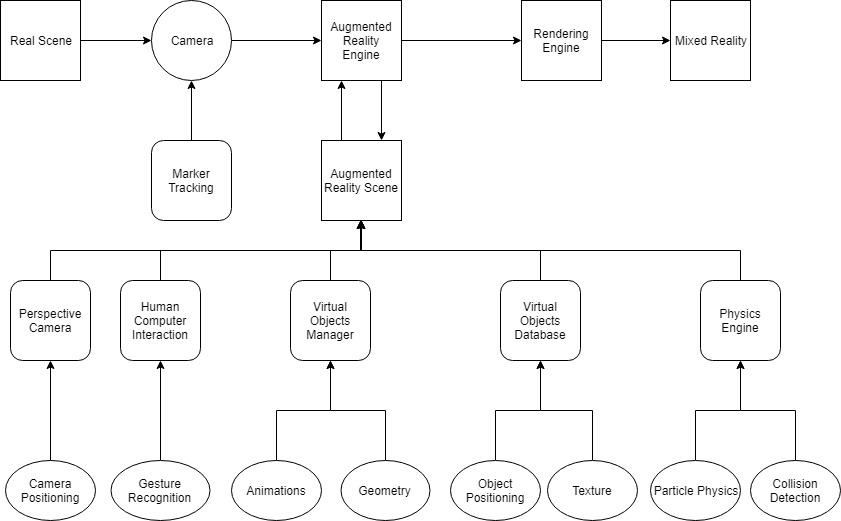
\includegraphics[width=\linewidth]{architecture.jpg}
	\caption{System Architecture.}
	\label{fig:system-architecture}
\end{figure}
\subsection{Interaction}
Using this virtual sandbox we are going to build the structures on a table-top environment that can be visualized in 3-D using AR technology. The structural components such as walls, columns, windows, doors, and pipings and electrical wires are included in the toolset that can be placed in the virtual scene by the user according to their requirements.To give the user a sense of freedom, The hand-tracking plays a major role in designing as it needs to be accurate and with utmost precision to provide a natural and interactive experience. Once the structure has been designed, various
simulations can be performed on the designed structure to understand the structural integrity.

The interaction of various simulated calamities used on the structural design are as follows:
\paragraph{Rain}  When taking a design into consideration, a structure should be well designed both inside and out. And due to the cohesive nature of water, it can be a major damage causing agent to the structure. As some materials absorb water and get weak over time. By simulating the effect of water on the materials used in construction we can better understand the integrity of a structure and find any weaknesses if present.

\paragraph{Wind}: It is helpful in simulating the effect of high altitude winds such as storms and hurricanes.This can also help us to create a better design by managing the ventilation areas, the flow of air in the building thus minimizing the damage to the structure.   

\paragraph{Floods}: Floods are a frequent disaster, occurring when water flows over the usual level in riverbeds or banks. Floods usually result from a combination of various unfavorable events, an especially significant one is a large amount of precipitation within a relatively short time. If precipitation falls onto a frozen, impermeable, or saturated surface, the riverbeds fill very quickly. Because they cannot drain the surplus water,
the water flows over the river channels.Therefore, the most appropriate method remains the selection of a suitable and safe location, in some places, damage can be reduced by erecting a building without a cellar or in an elevated location.

\paragraph{Lightning \& Fire}: Fire is a disaster that is not always caused by a natural phenomenon. It is natural only if it is caused by
lightning or some other natural process. Every year, several hundreds of buildings are affected by fire caused by lightning.Such fires can be practically reduced, thanks to developments in lighting and heating technology and the use of less flammable building materials. Simulation of the spread of fire over the structure can help us in placing safety exits that are easy to access and are unaffected by the fire.

\paragraph{Earth-quake}: Earthquakes are natural processes that affect people frequently and severely. The casualties and injuries are the result of destroyed buildings, fires, floods, uncontrolled leakage of hazardous substances into the environment, explosions and other changes are caused by the earthquakes. Earthquakes destroy or damage primarily older buildings. Even when the structures are built in line with earthquake safety regulations, they can still suffer from severe damage. Well-constructed and well-renovated buildings can reduce the impact to a minor range. By analyzing the structural weak points and using lightweight materials its impact can be reduced.

\section{Prototype System}
% TODO: Include Open Source Libraries %
As the project should be easily accessible, We've developed it using Web Technologies so that it can run on any device that has a web browser and is not limited by OS or Hardware.
Since it is a web application no installation is required and can be accessed anywhere.

\subsection{Frameworks, Tools used for development}
\subsubsection{Three.js} Three.js is a cross-browser JavaScript library/API used to create and display animated 3D computer graphics in a web browser. Three.js uses WebGL.
\subsubsection{AR.js}AR.js is efficient Augmented Reality for the web that also works well on mobile devices too. It is all in javascript and runs in any browser with WebGL and WebRTC. 
\subsubsection{A-Frame} A-Frame is a powerful entity-component framework that provides a declarative, extensible, and composable structure to three.js.
A-Frame’s core components include geometries, materials, lights, models, shadows, physics, motion capture and augmented reality.
\subsubsection{Tracking.js} The tracking.js library brings different computer vision algorithms and techniques into the browser environment. By using modern HTML5 specifications real-time color tracking, face detection, motion tracking is possible.
\begin{figure}
	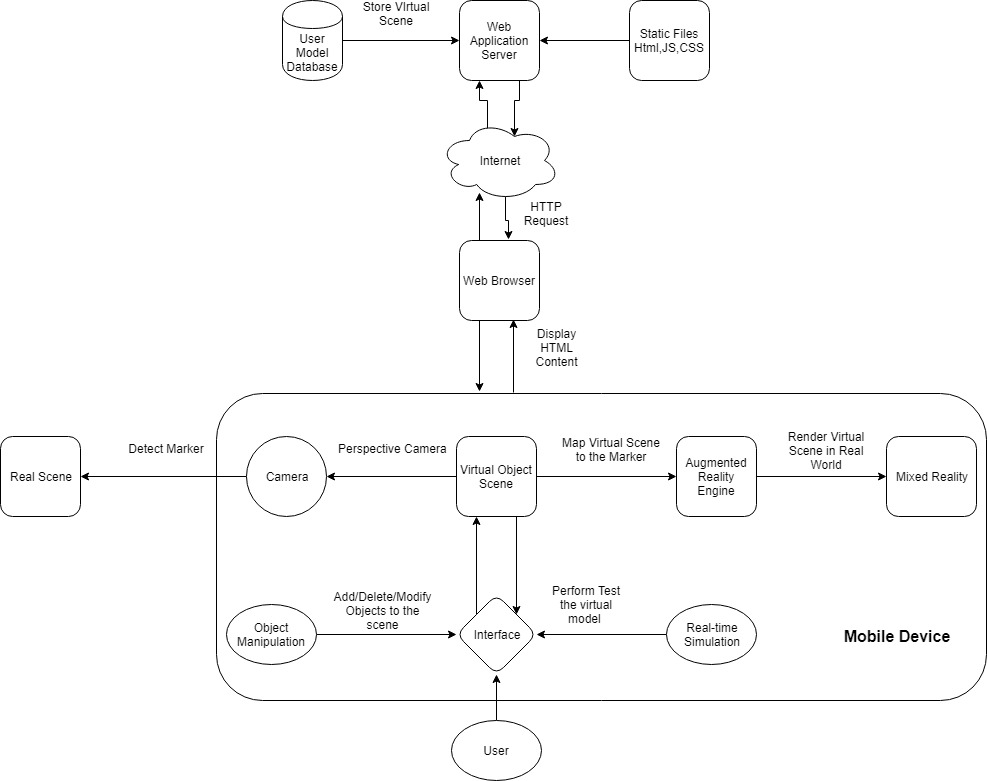
\includegraphics[width=\linewidth]{dataflow.jpg}
	\caption{Data Flow Diagram}
	\label{fig:data-flow}
\end{figure}
\subsection{Modules}
With the help of advanced augmented-reality technology such as computer vision and object recognition, the information about the surrounding real world of the user becomes interactive and able to be digitally manipulated. 
\subsubsection{Marker Tracking}
Marker-based AR uses a Camera and a visual marker to determine the center, orientation and range of its spherical coordinate system. Using a marker makes the application run faster as the object to detect is known beforehand.
\subsubsection{Gesture Recognition}
Interaction with the digital environment via hand gestures makes the experience quick and natural. Gestures to scale, manipulate or rotate the 3D Scene gives the user a sense of freedom.
\subsubsection{3D Scene Rendering}
Rendering the virtual model using WebGL and mapping it on the marker. Visual artifacts like shadows, lighting, texture, and distance are added to the final render that is displayed on the screen.
\subsubsection{3D Object Interaction}
The real space is used for data input, users perform gestures that are detected by the camera in real-time and the 3D virtual scene is projected onto the real environment reflecting the changes made by the user.

\subsubsection{Perspective Camera}
This camera mode is designed to mimic the way the human eye sees. It is the most common projection mode used for rendering a 3D scene. When there is camera movement the perspective of the 3D virtual scene is also changed accordingly
% TODO:Table %
\section{Conclusion}
This paper proposes a method of application of physics engine to perform realistic simulations to the architectural design in AR environment that allows the user to interact with ease.

In this paper, we have included several test cases for simulating the natural calamities on the design that helps in providing an in-depth analysis of the structural weak points. Based on this report we can then improve our design by altering the materials or layout of the structure.To realize physical interactions different physical attributes like structural integrity, gravity and dynamics are taken into consideration. 

In the future gesture recognition techniques for placing 3D objects in AR environment can make the experience more interactive and realistic.
Since simulations are very resource intensive tasks the performance can be improved in future by rendering the simulation using server-side GPU computing.

Thus the application of AR in the field of architecture, structural design will eventually be useful to the Architects, Students as the design process is more interactive and helps in creating high-quality designs that can be visualized as if it was present in the real world.

\bibliographystyle{unsrt}
\bibliography{references}
\end{document}